\documentclass{beamer}

\usepackage{préambule}

\newcommand{\IfSelectedNumber}[3]{
	\ifthenelse{\equal{#1}{50}}{}{
		\ifthenelse{
			\equal{#1}{11} \OR \equal{#1}{33} \OR \equal{#1}{14} \OR \equal{#1}{8} \OR \equal{#1}{42}
		}{#2}{#3}
	}
}

\newcommand{\IfSelectedComplementNumber}[3]{
	\ifthenelse{\equal{#1}{6}}{#2}{#3}
}

\begin{document}

\begin{frame}
	\small

	Règles du loto :
	\begin{enumerate}
		\item Une urne contient des boules numérotées de $1$ à $49$.

		      On effectue $5$ tirage dans cette urne, sans remise en jeu (chaque boule ne peut être tirée qu'une seule fois).
		\item On effectue ensuite un seul autre tirage, dit «complémentaire», dans une autre urne contenant des boules numérotées de 1 à 10.
	\end{enumerate}

	Pour gagner le gros lot au loto, il faut :
	\begin{itemize}
		\item Avoir coché les cinq numéros tirés à la première étape. L'ordre des numéros n'importe pas.
		\item Avoir coché le numéro complémentaire.
	\end{itemize}

	\begin{center}
		\uline{Exemple :}\vspace{0.5em}

		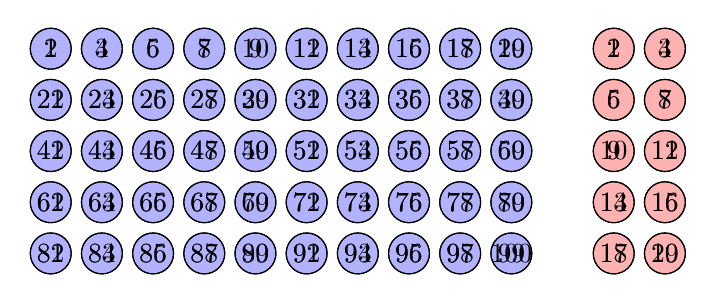
\begin{tikzpicture}[scale=0.65]
			\newcounter{Numero}
			\setcounter{Numero}{1}
			\foreach \y in {4,3,...,0} {
					\foreach \x in {0,...,9} {
							\IfSelectedNumber{\arabic{Numero}}{
								\draw[fill=blue!30] (\x,\y) circle (0.4);
								\node at (\x,\y) {\arabic{Numero}};
								\stepcounter{Numero}
							}{
								\node at (\x,\y) {\arabic{Numero}};
								\draw (\x,\y) circle (0.4);
								\stepcounter{Numero}
							}
						}
				}
			\setcounter{Numero}{1}
			\foreach \y in {4,3,...,0} {
					\foreach \x in {11,12} {
							\IfSelectedComplementNumber{\arabic{Numero}}{
								\draw[fill=red!30] (\x,\y) circle (0.4);
								\node at (\x,\y) {\arabic{Numero}};
								\stepcounter{Numero}
							}{
								\node at (\x,\y) {\arabic{Numero}};
								\draw (\x,\y) circle (0.4);
								\stepcounter{Numero}
							}
						}}
		\end{tikzpicture}
	\end{center}
\end{frame}

\end{document}